\documentclass{ximera}
\input{../preamble}
\addPrintStyle{..}
\begin{document}
\author{Alexander Holvoet}
\xmtitle]{Basis(sen) definiëren}{}

% Oefeningen: Coördinatentransformaties in ℝ²
% Gebaseerd op coordinate systems visualisatie

\begin{problem}
Beschouw de volgende twee coördinatenstelsels in $\mathbb{R}^2$: het zwarte coördinatenstelsel en het blauwe coördinatenstelsel. In de figuur zijn vijf punten aangeduid: $a$, $b$, $c$, $d$, en $e$.

\begin{center}
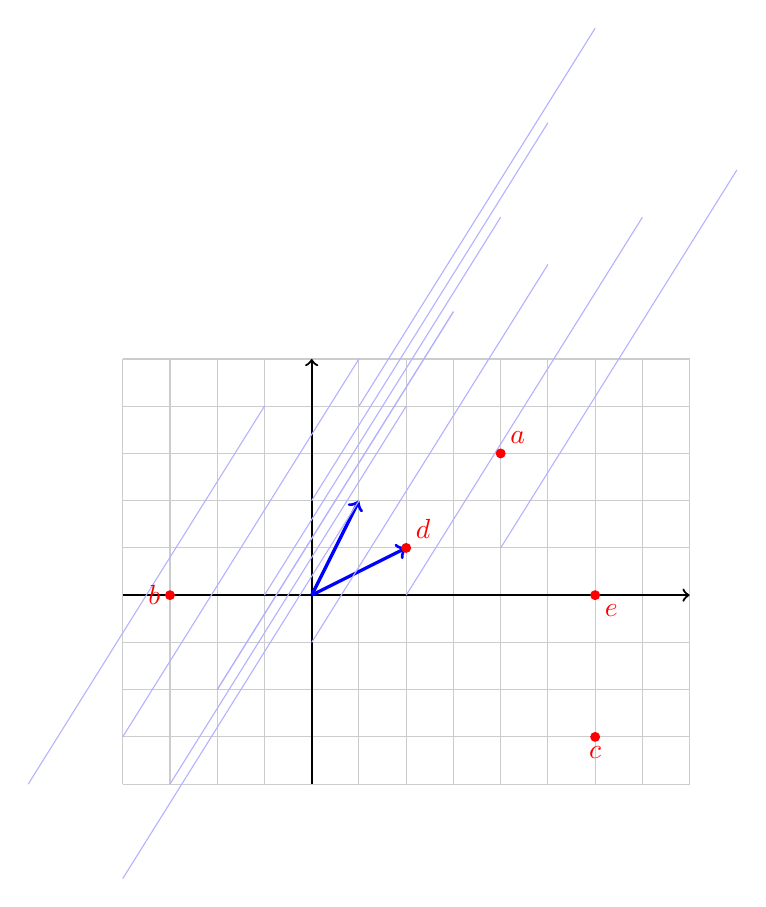
\begin{tikzpicture}[scale=0.6]
% Zwart coördinatenstelsel (standaard cartesiaans)
\draw[black!20, thin, step=1] (-4,-4) grid (8,5);
\draw[black, thick, ->] (-4,0) -- (8,0) node[right] {};
\draw[black, thick, ->] (0,-4) -- (0,5) node[above] {};

% Blauw coördinatenstelsel (geroteerd en geschaald)
% Blauwe basisvector 1: (2,1) in zwarte coördinaten
% Blauwe basisvector 2: (1,2) in zwarte coördinaten
\draw[blue, very thick, ->] (0,0) -- (2,1) node[midway, below right] {};
\draw[blue, very thick, ->] (0,0) -- (1,2) node[midway, above left] {};

% Blauwe rasterlijnen
\foreach \i in {-2,-1,0,1,2,3} {
  \draw[blue!30, thin] ({\i*2 - 2}, {\i*1 - 2}) -- ({\i*2 + 3}, {\i*1 + 6});
  \draw[blue!30, thin] ({\i*1 - 2}, {\i*2 - 2}) -- ({\i*1 + 3}, {\i*2 + 6});
}

% Punten
\fill[red] (4,3) circle (3pt) node[above right] {$a$};
\fill[red] (-3,0) circle (3pt) node[left] {$b$};
\fill[red] (6,-3) circle (3pt) node[below] {$c$};
\fill[red] (2,1) circle (3pt) node[above right] {$d$};
\fill[red] (6,0) circle (3pt) node[below right] {$e$};
\end{tikzpicture}
\end{center}

Schrijf de coördinaten van elk van de bovenstaande punten relatief ten opzichte van zowel het blauwe als het zwarte coördinatenstelsel.
\end{problem}

\begin{freeResponse}
Om de coördinaten te vinden, moeten we voor elk punt de afstand langs de basissen van beide coördinatenstelsels bepalen.

\textbf{Aanpak:} Gebruik de rasterlijnen om de componenten af te lezen in beide stelsels.

Uit de figuur lezen we (bij benadering):

\textbf{Punt a:}
\begin{itemize}
\item Zwart systeem: $(4, 3)$
\item Blauw systeem: $(2, 1)$
\end{itemize}

\textbf{Punt b:}
\begin{itemize}
\item Zwart systeem: $(-3, 0)$
\item Blauw systeem: $(-1, 2)$
\end{itemize}

\textbf{Punt c:}
\begin{itemize}
\item Zwart systeem: $(6, -3)$
\item Blauw systeem: $(3, -1)$
\end{itemize}

\textbf{Punt d:}
\begin{itemize}
\item Zwart systeem: $(2, 1)$
\item Blauw systeem: $(1, 0)$
\end{itemize}

\textbf{Punt e:}
\begin{itemize}
\item Zwart systeem: $(6, 0)$
\item Blauw systeem: $(3, 0)$
\end{itemize}

\textbf{Verificatie:} De punten die op een as liggen (zoals $e$ op de horizontale as) geven een nulcoördinaat in de andere richting.

\textbf{Mogelijke studentenfouten:}
\begin{itemize}
\item Verwarring over welke basis bij welk systeem hoort (basissen niet correct identificeren)
\item Verkeerde richting aflezen (mintekens verwisselen)
\item Vergeten dat de basissen verschillende lengtes kunnen hebben
\item De oorsprong van het blauwe systeem niet correct lokaliseren in het zwarte systeem
\end{itemize}
\end{freeResponse}

\begin{problem}
Bepaal een matrix die:
\begin{enumerate}
\item Punten van het blauwe coördinatenstelsel omzet naar punten in het zwarte coördinatenstelsel.
\item Punten van het zwarte coördinatenstelsel omzet naar punten in het blauwe coördinatenstelsel.
\end{enumerate}
\end{problem}

\begin{freeResponse}
\textbf{Conceptuele aanpak:} De transformatiematrix wordt gevormd door de basisvectoren van het ene systeem uit te drukken in het andere systeem.

\textbf{Deel a: Van blauw naar zwart}

We moeten de blauwe basisvectoren uitdrukken in zwarte coördinaten.

Uit de figuur zien we dat:
\begin{itemize}
\item De eerste blauwe basisvector (horizontale richting blauw) in zwarte coördinaten: $(2, 1)$
\item De tweede blauwe basisvector (verticale richting blauw) in zwarte coördinaten: $(1, 2)$
\end{itemize}

De transformatiematrix van blauw naar zwart is:
$$A_{b \to z} = \begin{pmatrix} 2 & 1 \\ 1 & 2 \end{pmatrix}$$

De kolommen zijn de blauwe basisvectoren uitgedrukt in het zwarte systeem.

\textbf{Verificatie met punt $a$:}
$$\begin{pmatrix} 2 & 1 \\ 1 & 2 \end{pmatrix} \begin{pmatrix} 2 \\ 1 \end{pmatrix} = \begin{pmatrix} 5 \\ 4 \end{pmatrix}$$

(Dit zou moeten kloppen met de zwarte coördinaten van punt $a$.)

\textbf{Deel b: Van zwart naar blauw}

Deze matrix is de inverse van de matrix hierboven:
$$A_{z \to b} = A_{b \to z}^{-1} = \begin{pmatrix} 2 & 1 \\ 1 & 2 \end{pmatrix}^{-1}$$

Bereken de inverse:
$$\det(A_{b \to z}) = 2 \cdot 2 - 1 \cdot 1 = 3$$

$$A_{z \to b} = \frac{1}{3} \begin{pmatrix} 2 & -1 \\ -1 & 2 \end{pmatrix} = \begin{pmatrix} 2/3 & -1/3 \\ -1/3 & 2/3 \end{pmatrix}$$

\textbf{Verificatie:} $A_{b \to z} \cdot A_{z \to b} = I$

\textbf{Mogelijke studentenfouten:}
\begin{itemize}
\item Rijen en kolommen verwisselen (basisvectoren als rijen schrijven in plaats van kolommen)
\item Vergeten dat de transformatie afhangt van de richting (blauw→zwart vs. zwart→blauw)
\item Verkeerde inverse berekenen (teken- of rekenfouten)
\item De basisvectoren verkeerd aflezen uit de figuur
\item Denken dat beide matrices hetzelfde zijn
\end{itemize}
\end{freeResponse}

\section*{Didactische Aanbevelingen}

\subsection*{1. Conceptontwikkeling}

\textbf{Van concreet naar abstract:}
\begin{itemize}
\item Begin met fysieke materialen: gebruik twee transparante rasters die gedraaid/geschaald ten opzichte van elkaar liggen
\item Laat studenten eerst punten plotten in beide systemen voordat ze matrices gebruiken
\item Maak de connectie met GPS-coördinaten vs. lokale kaartcoördinaten
\end{itemize}

\textbf{Visuele fundamenten:}
\begin{itemize}
\item Gebruik kleurcodering consequent (dit materiaal gebruikt zwart/blauw)
\item Laat studenten zelf coördinatenstelsels tekenen en basissen identificeren
\item Gebruik dynamische software (GeoGebra) om transformaties te visualiseren
\end{itemize}

\textbf{Connectie met voorkennis:}
\begin{itemize}
\item Koppel aan eerdere kennis over basissen en lineaire onafhankelijkheid
\item Verbind met vector optelling en scalaire vermenigvuldiging
\item Laat zien hoe dit generaliseert naar hogere dimensies
\end{itemize}

\subsection*{2. Differentiatie}

\textbf{Voor gevorderde studenten:}
\begin{itemize}
\item Vraag ze transformaties in 3D te beschouwen
\item Laat ze composities van transformaties onderzoeken
\item Onderzoek eigenschappen die invariant blijven onder coördinatentransformaties
\item Connectie met eigenvectoren: wanneer blijft een vector in dezelfde richting?
\end{itemize}

\textbf{Ondersteuning voor zwakkere studenten:}
\begin{itemize}
\item Geef eerst oefeningen met orthonormale stelsels (gemakkelijker af te lezen)
\item Gebruik stelsels die alleen geschaald zijn, niet geroteerd
\item Werk met hele getallen in plaats van breuken
\item Geef een stappenplan voor het aflezen van coördinaten
\end{itemize}

\textbf{Alternative oplossingsmethoden:}
\begin{itemize}
\item Algebraïsch: stelsel vergelijkingen opstellen
\item Geometrisch: gebruik maken van vectorprojecties
\item Numeriek: least-squares benadering bij meer dan 2 punten
\end{itemize}

\subsection*{3. Evaluatie}

\textbf{Procedurele vs. conceptuele beoordeling:}
\begin{itemize}
\item Procedureel: kunnen studenten de matrix correct opstellen en inverse berekenen?
\item Conceptueel: begrijpen ze waarom de kolommen basisvectoren zijn?
\item Conceptueel: kunnen ze uitleggen waarom inverse nodig is voor de omgekeerde richting?
\end{itemize}

\textbf{Veelvoorkomende foutpatronen:}
\begin{itemize}
\item Matrix transponeren in plaats van inverteren
\item Basis vectoren als rijen in plaats van kolommen
\item Oorsprong verkeerd lokaliseren
\item Kenteken fouten bij inverse berekening
\end{itemize}

\textbf{Rubric suggesties:}
\begin{itemize}
\item Correcte identificatie basisvectoren (30\%)
\item Juiste matrix opstelling (30\%)
\item Correcte inverse berekening (20\%)
\item Verificatie/controle (10\%)
\item Conceptueel begrip in uitleg (10\%)
\end{itemize}

\subsection*{4. Technologie-integratie}

\textbf{Visualisatie software:}
\begin{itemize}
\item GeoGebra: interactieve coördinatenstelsels
\item Desmos: transformaties visualiseren
\item Python met matplotlib: programmatisch transformaties toepassen
\end{itemize}

\textbf{Computationele verificatie:}
\begin{itemize}
\item NumPy voor matrix operaties en inverse berekening
\item Symbolische wiskunde (SymPy) voor exacte berekeningen
\item MATLAB/Octave voor grotere systemen
\end{itemize}

\textbf{Interactieve exploratie:}
\begin{itemize}
\item Laat studenten hun eigen coördinatenstelsels ontwerpen
\item Gebruik sliders om te zien hoe transformatiematrix verandert
\item Animaties van continue transformaties
\end{itemize}

\subsection*{5. Curriculaire Connecties}

\textbf{Wiskundige onderwerpen:}
\begin{itemize}
\item Lineaire algebra: basistransformaties, gelijkheidstransformaties
\item Analytische meetkunde: transformaties van krommen
\item Differentiaalvergelijkingen: fasevlak transformaties
\item Groepentheorie: transformatiegroepen
\end{itemize}

\textbf{Toepassingen:}
\begin{itemize}
\item Computer graphics: viewport transformaties
\item Robotica: coördinatentransformaties tussen gewrichten
\item GPS en kartografie: conversie tussen coördinatensystemen
\item Natuurkunde: referentiekaders (relativity, mechanica)
\item Data science: principale componentenanalyse (PCA)
\end{itemize}

\textbf{Historische context:}
\begin{itemize}
\item Descartes en de introductie van coördinaten
\item Einstein en coördinatentransformaties in relativiteit
\item Ontwikkeling van computergraphics in de 20e eeuw
\end{itemize}


\end{document}